\chapter{强化学习的神经科学} \label{chap:chap12}


神经科学是对神经系统的多学科研究:它们如何调节身体功能;控制行为;随着时间的推移,由于发展、学习和衰老而发生的变化;以及细胞和分子机制如何使这些功能成为可能。
强化学习最令人兴奋的方面之一是来自神经科学的越来越多的证据,证明人类和许多其他动物的神经系统实现的算法与强化学习算法惊人地对应。
本章的主要目的是解释这些相似之处,以及它们对动物奖励相关学习的神经基础的建议。


强化学习和神经科学之间最显著的联系点涉及多巴胺,这是一种深入参与哺乳动物大脑奖励处理的化学物质。
多巴胺似乎会将\textit{时间差分}误差传递给进行学习和决策的大脑结构。
\textit{多巴胺神经元活动的奖赏预测误差假说}表达了这种平行性,该假说是由计算强化学习和神经科学实验结果的汇聚引起的。
在本章中,我们讨论了这一假设,导致这一假设的神经科学发现,以及为什么它对理解大脑奖励系统有重要贡献。
我们还讨论了强化学习和神经科学之间的相似之处,这些相似之处不如\textit{多巴胺}/\textit{时间差分误差}的相似之处引人注目,但为思考动物基于回报的学习提供了有用的概念工具。
强化学习的其他元素有可能影响神经系统的研究,但它们与神经科学的联系仍相对未开发。
我们讨论了其中几个不断发展的联系,我们认为这些联系将随着时间的推移而变得越来越重要。


正如强化学习的早期历史所概述的,强化学习的许多方面都受到了神经科学的影响。
本章的第二个目标是让读者了解对我们贡献的强化学习方法关于大脑功能的想法。
从大脑功能的理论来看,强化学习的一些元素更容易理解。
\textit{资格迹}是强化学习的基本机制之一,它起源于突触的一种推测性质,突触是神经细胞(神经元)相互交流的结构。


在本章中,我们没有深入研究动物基于奖励的学习背后的神经系统的巨大复杂性:本章太短,我们不是神经科学家。
我们没有试图描述,甚至没有命名,许多大脑结构和通路,或任何分子机制,被认为与这些过程有关。
我们也没有公正地对待那些与强化学习非常一致的假设和模型的替代品。
该领域的专家之间存在分歧并不奇怪。
我们只能一窥这个引人入胜、不断发展的故事。
不过,我们希望本章能让你相信,一个非常富有成效的渠道已经出现,它将强化学习及其理论基础与动物基于奖励的学习的神经科学联系起来。


许多优秀的出版物涵盖了强化学习和神经科学之间的联系,其中一些我们在本章的最后一节中引用。
我们的处理与大多数处理不同,因为我们假设熟悉强化学习,但我们不假设了解神经科学。
我们首先简要介绍神经科学的概念,这些概念对于基本理解接下来的内容是必要的。



\section{神经科学基础} \label{sec:neuroscience_basics}

一些关于神经系统的基本信息有助于我们理解本章的内容。
我们后面提到的术语都是斜体字。
如果你已经掌握了神经科学的基本知识,跳过这一节就不会有问题。


\textit{神经元}是神经系统的主要组成部分,是专门利用电信号和化学信号处理和传递信息的细胞。
它们有多种形式,但神经元通常有一个细胞体、\textit{树突}和一个\textit{轴突}。
树突是从细胞体分支以接收来自其他神经元的输入(或者在感觉神经元的情况下也接收外部信号)的结构。
神经元的轴突是将神经元的输出传递给其他神经元(或肌肉或腺体)的纤维。
神经元的输出由一系列称为\textit{动作电位}的电脉冲组成,这些电脉冲沿着轴突传播。
动作电位也被称为\textit{脉冲},据说神经元在产生脉冲时会重新启动。
在神经网络模型中,通常使用实数来表示神经元的\textit{激活率},即某个单位时间内脉冲的平均数量。


神经元的轴突可以广泛分支,从而使神经元的动作电位达到许多目标。
神经元轴突的分支结构称为神经元轴突轴。
因为动作电位的传导是一个活跃的过程,与保险丝的燃烧没有什么不同,当动作电位到达轴突分支点时,它会“点亮”所有传出分支上的动作电位(尽管传播到分支有时会失败)。
因此,具有大轴突轴的神经元的活动可以影响许多靶位点。


\textit{突触}是一种通常位于轴突分支末端的结构,它介导一个神经元与另一个神经元的通信。
突触将信息从突触前神经元的轴突传递到突触后神经元的树突或细胞体。
除了少数例外,突触在突触前神经元的动作电位到达时会释放一种化学\textit{神经递质}。
(神经元之间直接电耦合的情况除外,但这里我们不关心这些。)
从突触突触前侧释放的神经递质分子扩散穿过突触间隙,即突触前末端和突触后神经元之间的非常小的空间,然后与突触后神经元表面的受体结合,以刺激或抑制其刺突生成活动,或以其他方式调节其行为。
一种特定的神经递质可能与几种不同类型的受体结合,每种受体对突触后神经元产生不同的影响。
例如,神经递质多巴胺至少有五种不同的受体类型可以影响突触后神经元。
许多不同的化学物质已被确定为动物神经系统中的神经递质。


当神经元似乎不受与实验者感兴趣的任务相关的突触输入的驱动时,例如,当神经元的活动与作为实验的一部分传递给受试者的刺激不相关时,神经元的背景活动是其活动水平,通常是其环速。
由于来自更宽网络的输入,或者由于神经元或其突触内的噪声,背景活动可能是不规则的。
有时,背景活动是神经元固有的动态过程的结果。
与背景活动相比,神经元的阶段性活动由通常由突触输入引起的脉冲活动爆发组成。
缓慢且经常以分级方式变化的活动,无论是否作为背景活动,都被称为神经元的\textit{强直性}活动。


突触释放的神经递质影响突触后神经元的强度或有效性是突触的有效性。
神经系统可以通过经验改变的一种方式是通过突触前和突触后神经元活动组合引起的突触能力的改变,有时还通过神经调节剂的存在,神经调节剂是一种具有除直接快速兴奋或抑制之外或除直接快速激励或抑制之外的作用的神经递质。


大脑包含几个不同的神经调控系统,由具有广泛分支轴突轴的神经元簇组成,每个系统使用不同的神经递质。
神经调控可以改变神经回路的功能,介导动机、唤醒、注意力、记忆、情绪、情绪、睡眠和体温。
重要的是,神经调节系统可以分布标量信号,如强化信号,以改变对学习至关重要的广泛分布部位突触的操作。


突触效应改变的能力称为\textit{突触可塑性}。
它是负责学习的主要机制之一。
通过学习算法调整的参数或权重对应于突触。
正如我们下面详细介绍的那样,通过神经调节剂多巴胺调节突触可塑性是大脑如何实现本书中描述的许多学习算法的一种合理机制。


\section{奖励信号、强化信号、值和预测误差}

神经科学和计算强化学习之间的联系始于大脑中的信号与在强化学习理论和算法中发挥重要作用的信号之间的相似之处。
在有限马尔可夫决策过程中,任何学习目标导向行为的问题都可以归结为代表行动、状态和奖励的三个信号。
然而,为了解释神经科学和强化学习之间的联系,我们必须不那么抽象,而是考虑在某些方面与大脑中的信号相对应的其他强化学习信号。
除了奖励信号之外,这些信号还包括强化信号(我们认为这与奖励信号不同)、价值信号和传达预测误差的信号。
当我们以这种方式通过信号的函数来标记信号时,我们是在强化学习理论的背景下进行的,在该理论中,信号对应于方程或算法中的一个项。
另一方面,当我们提到大脑中的信号时,我们指的是一种生理事件,如动作电位的爆发或神经递质的分泌。
用神经信号的功能来标记神经信号,例如将多巴胺神经元的阶段性活动称为强化信号,意味着神经信号的行为类似于相应的理论信号,并被推测为其功能类似。



揭示这些对应关系的证据涉及许多挑战。
与奖励处理相关的神经活动几乎可以在大脑的每一个部位找到,并且很难明确地解释结果,因为不同的奖励相关信号的表示往往彼此高度相关。
实验需要仔细设计,以允许一种类型的奖励相关信号以任何程度的确定性与其他信号或与奖励处理无关的大量其他信号区分开来。
尽管存在这些分歧,但已经进行了许多实验,目的是将强化学习理论和算法的各个方面与神经信号相协调,并建立了一些令人信服的联系。
为了准备研究这些链接,在本节的其余部分中,我们提醒读者根据强化学习理论,各种与奖励相关的信号意味着什么。


在上一章末尾的术语评论中,我们说过 $ R_t $ 就像动物大脑中的奖励信号,而不是动物环境中的物体或事件。
在强化学习中,奖励信号(以及智能体的环境)定义了强化学习智能体试图解决的问题。
从这方面来说,$ R_t $ 就像动物大脑中的信号,将主要奖励分配到整个大脑的各个部位。
但动物大脑中不太可能存在像 $ R_t $ 这样单一的主奖励信号。
最好将 $ R_t $ 视为一个抽象概念,它总结了大脑中许多系统生成的大量神经信号的总体影响,这些系统评估感觉和状态的奖励或惩罚质量。


强化学习中的\textit{强化信号}与奖励信号不同。
强化信号的功能是指导学习算法在智能体的策略、价值估计或环境模型中做出的改变。
例如,对于时间差分方法,时间 $ t $ 时的强化信号是时间差分误差 $ \delta_{t-1} = R_t + \gamma V(S_t) - V(S_{t-1})$。
某些算法的强化信号可能只是奖励信号,但对于大多数算法,我们认为强化信号是通过其他信息调整的奖励信号,例如 时间差分误差中的值估计。


状态值或动作值(即 $ V $ 或 $ Q $)的估计指定从长远来看对智能体来说是好是坏。
它们是对智能体未来预期累积的总奖励的预测。
智能体通过选择导致具有最大估计状态值的状态的动作,或者通过选择具有最大估计动作值的动作来做出好的决策。


预测误差衡量预期信号或感觉与实际信号或感觉之间的差异。
\textit{奖励预测误差}专门衡量预期和收到的奖励信号之间的差异,当奖励信号大于预期时为正,否则为负。 
时间差分误差是特殊类型的\textit{奖励预测误差},它表明当前和早期的长期奖励预期之间存在差异。
当神经科学家提到\textit{奖励预测误差}时,他们通常(尽管并非总是)指的是时间差分 \textit{奖励预测误差},我们在本章中简称为时间差分误差。
同样在本章中,时间差分误差通常是不依赖于动作的误差,这与 Sarsa 和 Q-学习等算法在学习动作值时使用的时间差分误差相反。
这是因为最著名的神经科学链接是用无动作时间差分误差来表述的,但我们并不意味着排除涉及依赖动作的时间差分误差的可能的类似链接。
(时间差分误差对于预测奖励以外的信号也很有用,但我们在这里不关心这种情况\cite{modayil2014prediction}。)


人们可以就神经科学数据和这些理论上定义的信号之间的联系提出许多问题。
观察到的信号是否更像是奖励信号、价值信号、预测误差、强化信号,还是完全不同的东西?
如果它是一个误差信号,它是奖励预测误差、时间差分误差还是像\textit{雷斯科拉-瓦格纳模型}误差这样的更简单的误差?
如果是时间差分误差,它是否取决于 Q-学习或 Sarsa 的 时间差分误差之类的操作?
如上所述,探测大脑来回答此类问题是极其困难的。
但实验证据表明,一种神经递质,特别是神经递质多巴胺,向奖励预测误差发出信号,并且进一步,产生多巴胺的神经元的阶段性活动实际上传达了时间差分误差(有关阶段性活动的定义,请参见第~\ref{sec:neuroscience_basics}~节)。
这一证据导致了\textit{多巴胺神经元活动的奖励预测误差假设},我们接下来将对此进行描述。


\section{奖励预测误差假设}

多巴胺神经元活动的奖励预测误差假说提出,哺乳动物中产生多巴胺的神经元的阶段性活动的功能之一是将预期未来奖励的旧估计和新估计之间的误差传递给整个大脑的目标区域。
Montague\cite{montague1996framework}首先明确提出了这一假设(尽管没有用这些确切的措辞),他们展示了强化学习中的时间差分误差概念如何解释哺乳动物多巴胺神经元阶段性活动的许多特征。
得出这一假设的实验是在 20 世纪 80 年代和 90 年代初在神经科学家\textit{沃尔夫勒姆$\cdot$舒尔茨}的实验室进行的。
第~\ref{sec:experimental_support}~节描述了这些有影响力的实验,第~\ref{sec:td_dopamine}~节解释了这些实验的结果如何与时间差分误差保持一致,本章末尾的参考文献和历史评论部分包括围绕这一有影响力的假设的发展的文献指南。


Montague\cite{montague1996framework}等人将经典条件反射的时间差分模型的时间差分误差与经典条件反射实验中产生多巴胺的神经元的相位活动进行了比较。
回想一下~\ref{sec:classical_conditioning}~节,经典调节的时间差分模型基本上是具有线性函数近似的半梯度下降 TD($ \lambda $) 算法。
Montague等人做出了几个假设来进行这种比较。
首先,由于时间差分误差可以是负的,但神经元不能有负的激活率,他们假设多巴胺神经元活动对应的量是 $ \delta_{t-1} + b_t $,其中$ b_t $是神经元的背景激活率。
负时间差分误差对应于多巴胺神经元的激活率下降到其背景速率以下。



需要第二个假设,关于每个经典条件反射试验中访问的状态以及它们如何表示为学习算法的输入。
这与我们在~\ref{sec:td_simulation}~节中针对时间差分模型讨论的问题相同。 
Montague等人选择了\textit{全串行复合}表示,如图~\ref{fig:11_1}~左栏所示,但短期内部信号序列持续到\textit{非条件刺激}开始,这里是非零奖励信号的到来。
这种表示允许时间差分误差模拟这样一个事实:多巴胺神经元活动不仅预测未来的奖励,而且对奖励预计到达的预测提示之后的时间也很敏感。
必须有某种方法来跟踪感官提示和奖励到来之间的时间。
如果刺激启动一系列内部信号,并在刺激结束后继续,并且如果刺激后的每个时间步都有不同的信号,则刺激后的每个时间步都由不同的状态表示。
因此,时间差分误差与状态相关,可能对试验中事件的时间安排很敏感。


在使用有关背景激活率和输入表示的这些假设的模拟试验中,时间差分模型的时间差分误差与多巴胺神经元相位活动非常相似。
预览我们在下面第~\ref{sec:experimental_support}~节中对这些相似性的详细描述,时间差分误差与多巴胺神经元活动的以下特征相似:
1)多巴胺神经元的阶段性反应仅在奖励事件不可预测时发生;
2)在学习早期,奖励之前的中性线索不会引起实质性的阶段性多巴胺反应,但随着学习的继续,这些线索获得预测价值并引发阶段性多巴胺反应;
3)如果更早的提示可靠地先于已经获得预测值的提示,则阶段性多巴胺反应会转移到较早的提示,而停止等待较晚的提示;
3)如果在学习之后,预测的奖励事件被忽略,多巴胺神经元的反应在奖励事件的预期时间之后不久就会降低到其基线水平以下。


尽管\textit{舒尔茨}及其同事的实验中监测到的每个多巴胺神经元并非都以所有这些方式表现,但大多数监测神经元的活动与时间差分误差之间的惊人对应关系为奖励预测误差假说提供了强有力的支持。
然而,在某些情况下,基于假设的预测与实验中观察到的结果并不相符。
输入表示的选择对于时间差分误差与多巴胺神经元活动的一些细节的匹配程度至关重要,特别是有关多巴胺神经元响应时间的细节。
关于时间差分学习的输入表示和其他特征,人们提出了不同的想法,其中一些我们在下面讨论,以使时间差分误差更好地处理数据,尽管主要的相似之处与 Montague 等人用过的\textit{全串行复合}表示相似。
总体而言,奖励预测误差假说已得到研究基于奖励的学习的神经科学家的广泛接受,并且事实证明,面对神经科学实验不断积累的结果,它具有显着的弹性。


为了准备我们对支持奖励预测误差假说的神经科学实验的描述,并提供一些背景以便可以理解该假说的重要性,我们接下来介绍一些关于多巴胺的已知知识,以及它影响的大脑结构,以及它如何参与基于奖励的学习。


\section{多巴胺}

多巴胺作为神经递质由神经元产生,其细胞体主要位于哺乳动物中脑的两个神经元簇:\textit{黑质致密部}和\textit{腹侧被盖区}。
多巴胺在哺乳动物大脑的许多过程中发挥着重要作用。
其中最突出的是动机、学习、行动选择、大多数形式的成瘾以及精神分裂症和帕金森病。
多巴胺被称为神经调节剂,因为它除了直接快速兴奋或抑制目标神经元之外还执行许多功能。
尽管关于多巴胺的功能及其细胞效应的细节仍有很多未知之处,但很明显,它对于哺乳动物大脑中的奖励处理至关重要。
多巴胺并不是唯一参与奖励处理的神经调节剂,它在厌恶情况(惩罚)中的作用仍然存在争议。
多巴胺在非哺乳动物中也可以发挥不同的作用。
但没有人怀疑多巴胺对于哺乳动物(包括人类)的奖励相关过程至关重要。


早期的传统观点认为,多巴胺神经元向与学习和动机有关的多个大脑区域广播奖励信号。
这一观点源自 James Olds 和 Peter Milner 1954 年发表的一篇著名论文,该论文描述了电刺激对大鼠大脑某些区域的影响。
他们发现,对特定区域的电刺激在控制老鼠的行为方面起到了非常强大的奖励作用:“……通过这种奖励对动物行为的控制是极端的,可能超过以前在动物实验中使用的任何其他奖励。”\cite{olds1954positive}
后来的研究表明,刺激最有效地产生这种奖赏效应的位点会直接或间接地兴奋多巴胺通路,而这些通路通常会受到自然奖赏刺激的兴奋。
在人类受试者中也观察到了与大鼠相似的效应。
这些观察结果强烈表明多巴胺神经元活动发出奖励信号。


但是,如果奖励预测误差假设是正确的(即使它只解释了多巴胺神经元活动的某些特征)这种多巴胺神经元活动的传统观点并不完全正确:
多巴胺神经元的阶段性反应发出奖励预测错误的信号,而不是奖励本身。
用强化学习的术语来说,多巴胺神经元在时间 $ t $ 的相位响应对应于 $ \delta_{t-1} = R_t + \gamma V(S_t) - V(S_{t-1}) $,而不是 $ R_t $。


强化学习理论和算法有助于协调奖励预测误差观点与多巴胺信号奖励的传统观念。
在我们在本书中讨论的许多算法中,它起着强化信号的作用,这意味着它是学习的主要驱动力。
例如,$ \delta $是经典条件反射时间差分模型中的关键因素,是\textit{参与者-评论家}架构中的价值函数和策略的强化信号(第~\ref{sec:neural_ac}~节)。
动作依赖形式是 Q 学习和 Sarsa 的强化信号。
奖励信号 $ R_t $ 是 $ \delta_{t-1} $ 的关键组成部分,但它并不是其在这些算法中的强化效果的完全决定因素。
附加项 $ \gamma V(S_t) - V(S_{t-1}) $ 是 $ \delta_{t-1} $ 的高阶强化部分,即使奖励发生($ R_t \neq 0 $),如果奖励完全预测,时间差分误差也可以保持沉默。(在下面第~\ref{sec:td_dopamine}~节中有完整解释)。


事实上,仔细观察 Olds 和 Milner 1954 年的论文就会发现,它主要是关于电刺激在仪器调节任务中的强化作用。
电刺激不仅通过多巴胺对动机的影响激发了老鼠的行为,还使老鼠很快学会了通过按下杠杆来刺激自己,而它们会经常长时间这样做。
电刺激触发的多巴胺神经元的活动增强了大鼠的杠杆按压。


最近使用光遗传学方法的实验证实了多巴胺神经元的相位反应作为强化信号的作用。
这些方法使神经科学家能够在清醒行为动物中以毫秒为单位精确控制所选神经元类型的活动。
光遗传学方法将光敏蛋白引入选定的神经元类型中,以便可以通过激光的灰烬激活或沉默这些神经元。
第一个使用光遗传学方法研究多巴胺神经元的实验表明,在小鼠体内产生多巴胺神经元阶段性激活的光遗传学刺激足以使小鼠更喜欢接受刺激的室的一侧,而不是接受刺激的室的另一侧 无刺激或频率较低的刺激\cite{tsai2009phasic}。
在另一个例子中\cite{steinberg2013causal}使用多巴胺神经元的光遗传学激活,在预期奖励刺激的时间在大鼠中产生多巴胺神经元活动的人工爆发,但在多巴胺神经元活动正常暂停时却忽略了奖励刺激。
当这些停顿被人工爆发所取代时,当反应通常由于缺乏强化而减少时(在灭绝试验中),反应就会持续,而当反应通常由于已经预测到奖励而被阻止时,学习就会被启用(阻塞范式; 第~\ref{sec:blocking_higher_order}~节)。


多巴胺增强功能的额外证据来自于水果的光遗传学实验,但在这些动物中,多巴胺的作用与其在哺乳动物中的作用相反:光触发的多巴胺神经元活动爆发就像电击足部一样增强回避行为 ,至少对于激活的多巴胺神经元群体而言\cite{claridge2009writing}。
尽管这些光遗传学实验都没有表明相位多巴胺神经元活动特别像时间差分误差,但它们令人信服地证明了相位多巴胺神经元活动就像算法中的强化信号一样(或者可能像水果中的负行为) 用于预测(经典条件反射)和控制(仪器条件反射)。


多巴胺神经元特别适合向大脑的许多区域广播强化信号。
这些神经元具有巨大的轴突乔木,每个神经元释放的多巴胺的突触位点比典型神经元的轴突多出 100 至 1,000 倍。
图~\ref{fig:12_1}~显示了单个多巴胺神经元的轴突,其细胞体位于大鼠大脑的\textit{黑质致密部}中。
\textit{黑质致密部}或\textit{中脑腹侧被盖区}多巴胺神经元的每个轴突在目标大脑区域的神经元树突上产生大约 500,000 个突触接触。


\begin{figure}[!htb]
	\centering
	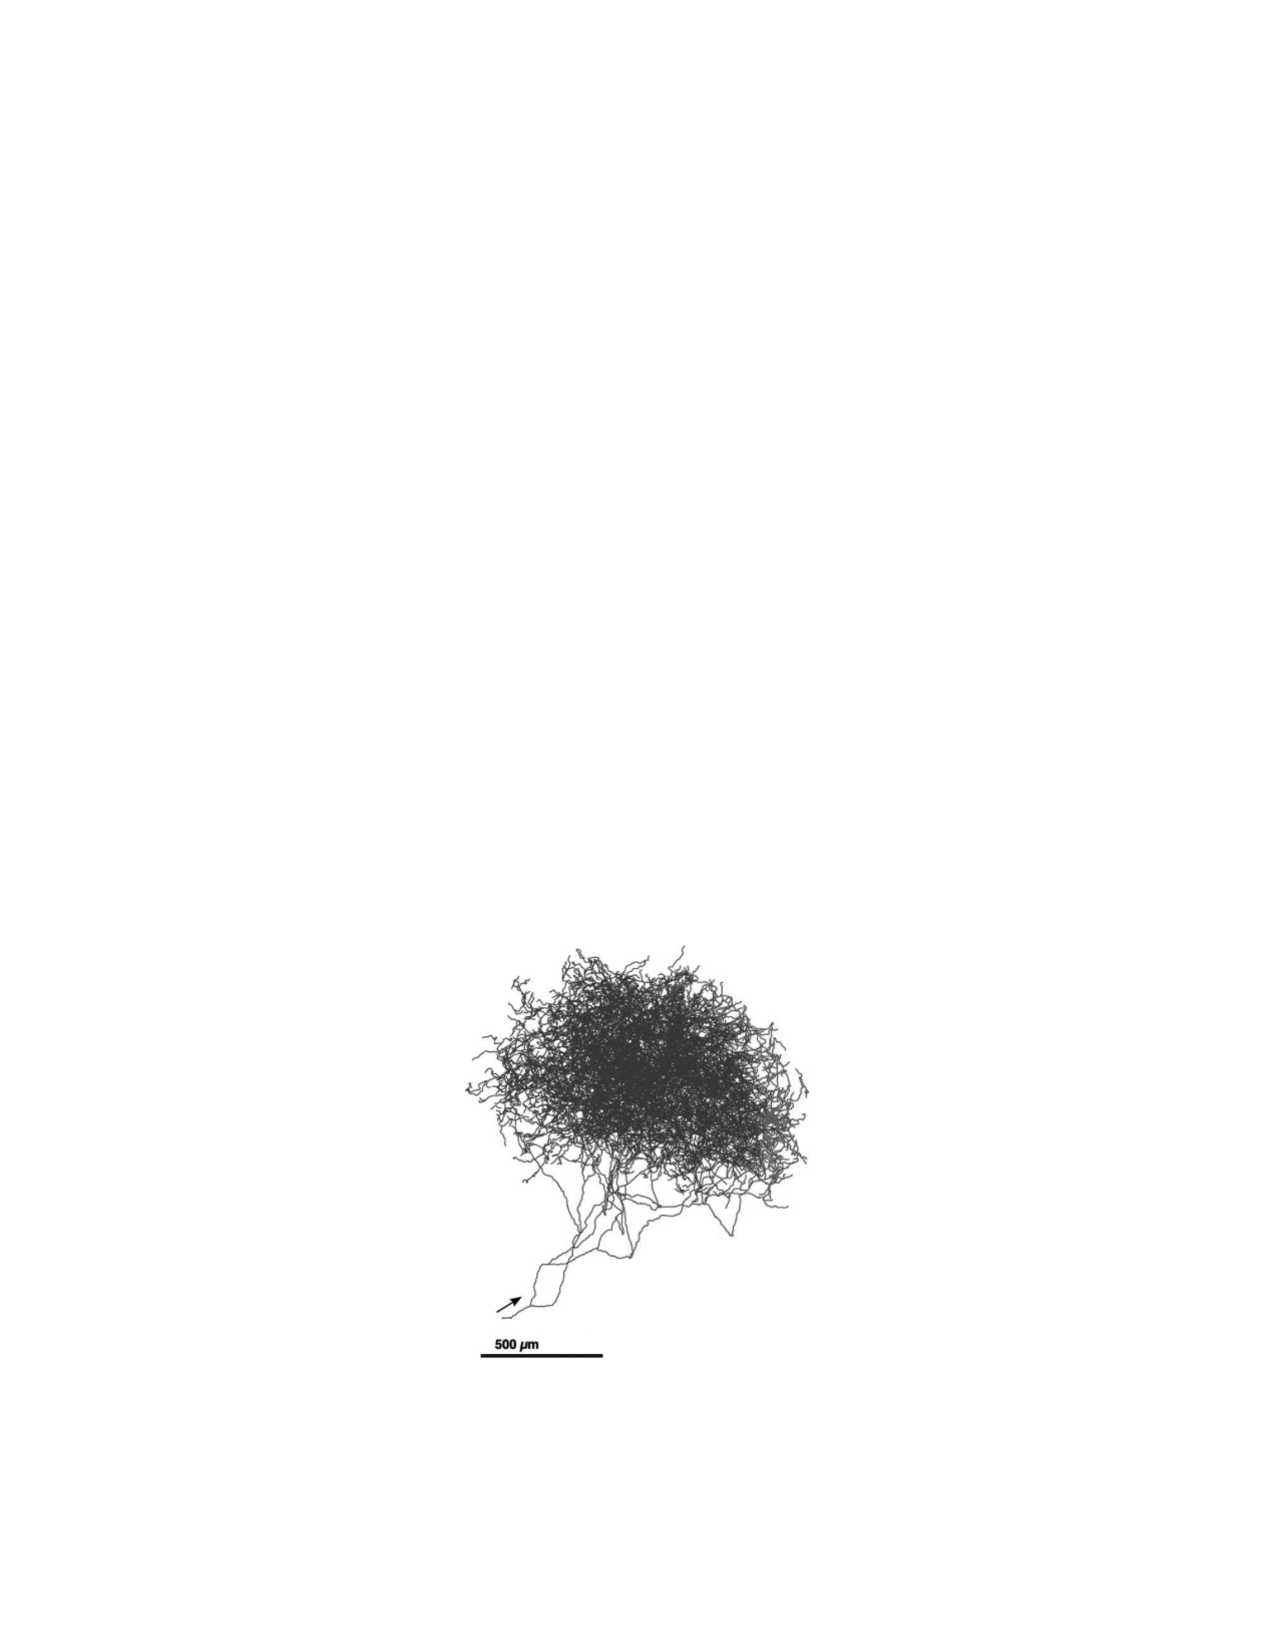
\includegraphics[width=0.5\linewidth]{chap12/fig_12_1}
	\caption{产生多巴胺作为神经递质的单个神经元的轴突乔木,其细胞体位于大鼠大脑的\textit{黑质致密部}中。
		这些轴突与目标大脑区域中的大量神经元树突进行突触接触。 \label{fig:12_1}}
\end{figure}


如果多巴胺神经元像强化学习那样广播强化信号,那么由于这是一个标量信号,即单个数字,因此\textit{黑质致密部}和\textit{中脑腹侧被盖区}中的所有多巴胺神经元将被期望或多或少相同地激活,以便它们近乎同步地行动,向轴突目标的所有部位发送相同的信号。 
尽管人们普遍认为多巴胺神经元确实像这样一起行动,但现代证据指出了更复杂的情况,即不同的多巴胺神经元亚群对输入的反应不同,具体取决于它们发送信号的结构和不同的结构。
这些信号以不同的方式作用于其目标结构。
多巴胺除了发出\textit{奖励预测误差}信号之外还有其他功能,即使对于发送\textit{奖励预测误差}信号的多巴胺神经元来说,根据这些结构在产生强化行为中所扮演的角色,将不同的\textit{奖励预测误差}发送到不同的结构也是有意义的。
这超出了我们在本书中详细讨论的范围,但从强化学习的角度来看,向量值\textit{奖励预测误差}信号是有意义的,因为决策可以分解为单独的子决策,或者更一般地说,作为解决问题的结构版本的一种方法。
信用分配问题:如何在可能参与制定决策的许多组成结构中分配决策成功的功劳(或失败的责任)?
我们在下面的~\ref{sec:collective_rl}~节中对此进行了更多讨论。


大多数多巴胺神经元的轴突与额叶皮层和基底神经节中的神经元进行突触接触,这些区域是大脑中参与随意运动、决策、学习和认知功能(例如计划)的区域。
由于大多数将多巴胺与强化学习相关的想法都集中在基底神经节上,并且多巴胺神经元的连接在那里特别密集,因此我们在这里重点关注基底神经节。
基底神经节是位于前脑底部的神经元群或细胞核的集合。 基底神经节的主要输入结构称为纹状体。
基本上所有的大脑皮层以及其他结构都向纹状体提供输入。
皮层神经元的活动传达了有关感觉输入、内部状态和运动活动的大量信息。
皮质神经元的轴突与纹状体主要输入/输出神经元的树突进行突触接触,称为中棘神经元。
纹状体的输出通过其他基底神经节核和丘脑循环回皮层的额叶区域和运动区域,使纹状体能够影响运动、抽象决策过程和奖励处理。
纹状体的两个主要细分对于强化学习很重要:背侧纹状体,主要参与影响动作选择;
腹侧纹状体,被认为对奖励处理的不同方面至关重要,包括将情感价值分配给感觉。



中型多刺神经元的树突上覆盖着刺,皮层神经元的轴突在其尖端进行突触接触。
与这些棘进行突触接触的还有多巴胺神经元的轴突(图~\ref{fig:12_2})。
这种排列汇集了皮质神经元的突触前活动、中型多棘神经元的突触后活动以及多巴胺神经元的输入。
这些刺上实际发生的事情很复杂并且尚未完全了解。
图~\ref{fig:12_2}~通过显示两种类型的多巴胺受体、谷氨酸受体|皮质输入的神经递质|以及各种信号相互作用的多种方式暗示了复杂性。
但越来越多的证据表明,从皮质到纹状体通路上的突触(神经科学家称之为皮层纹状体突触)的效率变化很大程度上取决于适当定时的多巴胺信号。



\begin{figure}[!htb]
	\centering
	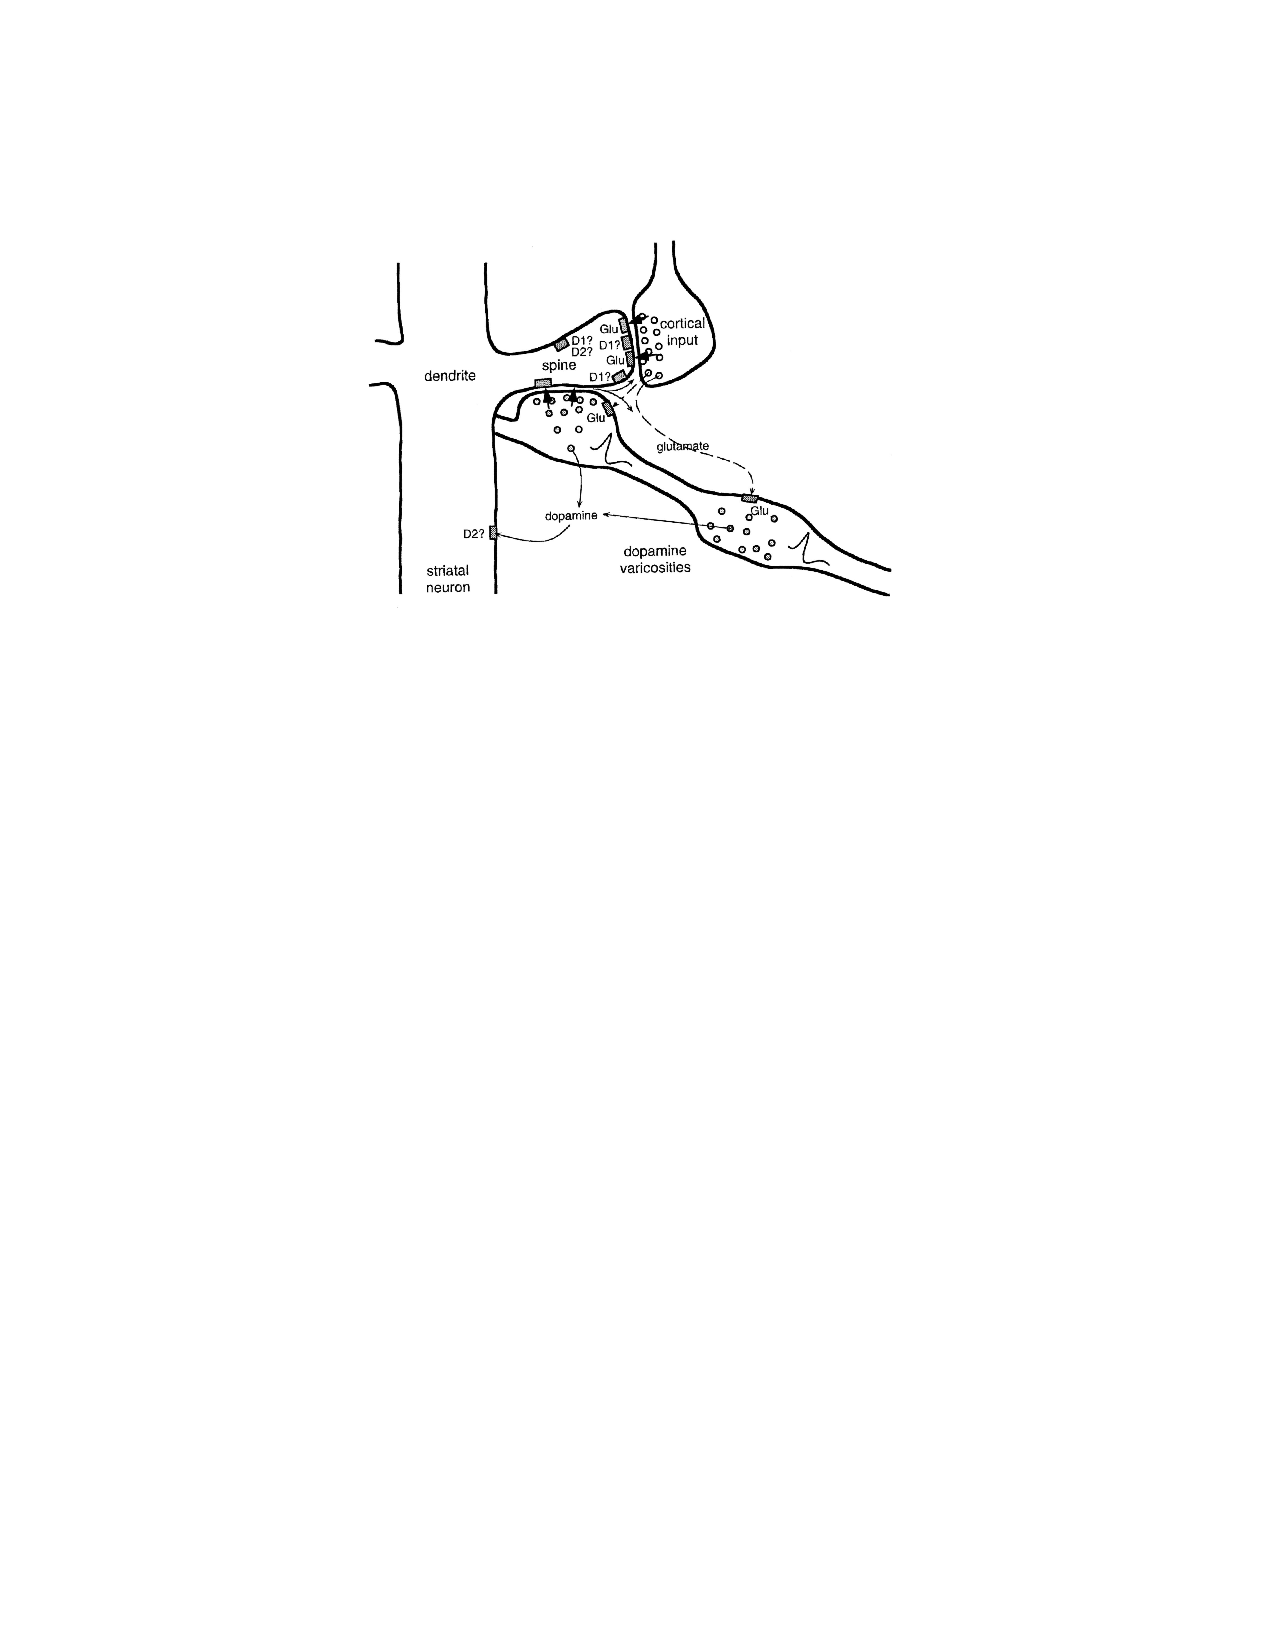
\includegraphics[width=0.5\linewidth]{chap12/fig_12_2}
	\caption{纹状体神经元的脊柱显示来自皮质和多巴胺神经元的输入。
		皮层神经元的轴突通过皮质纹状体突触影响纹状体神经元,在覆盖纹状体神经元树突的棘尖释放神经递质谷氨酸。
		显示 VTA 或 SNpc 多巴胺神经元的轴突经过脊柱(从右下)。
		该轴突上的“多巴胺静脉曲张”在脊柱干处或附近释放多巴胺,其排列将皮质的突触前输入、纹状体神经元的突触后活动和多巴胺结合在一起,使得几种类型的学习规则控制可塑性成为可能。
		多巴胺神经元的每个轴突与大约 500,000 个棘突的茎部进行突触接触,这里通过其他神经递质途径和多种受体类型(例如多巴胺通过的 D1 和 D2 多巴胺受体)显示了我们讨论中省略的一些复杂性。
		可以对棘和其他突触后部位产生不同的影响,摘自《神经生理学杂志》,W. Schultz,第 80 卷,1998 年,第 10 页。
		\label{fig:12_2}}
\end{figure}



\section{奖励预测误差假设的实验支持} \label{sec:experimental_support}

多巴胺神经元对强烈的、新颖的或意想不到的视觉和听觉刺激做出反应,这些刺激会引发眼睛和身体的运动,但它们的活动很少与运动本身相关。
这是令人惊讶的,因为多巴胺神经元的退化是帕金森病的一个原因,帕金森病的症状包括运动障碍,特别是自发运动的缺陷。
由于多巴胺神经元活动与刺激触发的眼睛和身体运动之间的微弱关系,Romo 和 Schultz (1990) 以及 Schultz 和 Romo (1990) 通过记录多巴胺神经元和肌肉的活动,迈出了奖励预测误差假说的第一步 当猴子移动手臂时进行活动。


他们训练两只猴子,当猴子看到并听到垃圾箱的门打开时,将手伸入装有一点苹果、一块饼干或葡萄干的垃圾箱。
然后猴子就可以抓住食物并将其送到嘴里。
当猴子擅长这项工作后,它又接受了另外两项任务的训练。
第一项任务的目的是观察当运动自发时多巴胺神经元会做什么。
箱子是开着的,但从上面盖住了,这样猴子就看不到里面的东西,但可以从下面伸手进去。
没有出现任何触发刺激,在猴子伸手去拿食物并吃掉后,实验者通常(尽管并非总是如此)在猴子看不见的情况下,将食物粘在一根坚硬的金属丝上,以取代垃圾箱中的食物。
在这里,罗莫和舒尔茨监测到的多巴胺神经元的活动与猴子的运动无关,但每当猴子第一次接触食物时,这些神经元中的很大一部分都会产生阶段性反应。
当猴子只触摸电线或在没有食物的情况下探索垃圾箱时,这些神经元不会做出反应。
这是神经元对食物而不是任务的其他方面做出反应的有力证据。


罗莫和舒尔茨的第二个任务的目的是看看当刺激触发运动时会发生什么。
这项任务使用了一个带有可移动盖子的不同垃圾箱。
垃圾箱打开的景象和声音引发了向垃圾箱伸出手的动作。
在这种情况下,罗莫和舒尔茨发现,经过一段时间的训练,多巴胺神经元不再对食物的触摸做出反应,而是对食物箱盖打开的视觉和声音做出反应。
这些神经元的阶段性反应已经从奖励本身转变为预测奖励可用性的刺激。
在后续研究中,罗莫和舒尔茨发现,他们监测的大多数多巴胺神经元的活动在行为任务背景之外对垃圾箱打开的景象和声音没有反应。
这些观察结果表明,多巴胺神经元既不响应运动的启动,也不响应刺激的感觉特性,而是发出奖励期望的信号。


Schultz 的小组进行了许多涉及 SNpc 和 VTA 多巴胺神经元的其他研究。
一系列特定的实验具有重要意义,表明多巴胺神经元的相位反应对应于 TD 误差,而不是像 Rescorla{Wagner 模型 (14.3) 中的那些更简单的误差。
在第一个实验中(Ljungberg、Apicella 和 Schultz,1992),猴子被训练在灯光亮起后按下杠杆作为“触发提示”,以获得一滴苹果汁。
正如罗莫和舒尔茨之前观察到的那样,许多多巴胺神经元最初对奖励|果汁滴做出反应(图~\ref{fig:12_3},上图)。
但随着训练的继续,许多神经元失去了奖励反应,并产生了对预测奖励的光照射的反应(图~\ref{fig:12_3},中图)。
随着持续的训练,按下杠杆的速度变得更快,而对触发信号做出反应的多巴胺神经元的数量却减少了。


\begin{figure}[!htb]
	\centering
	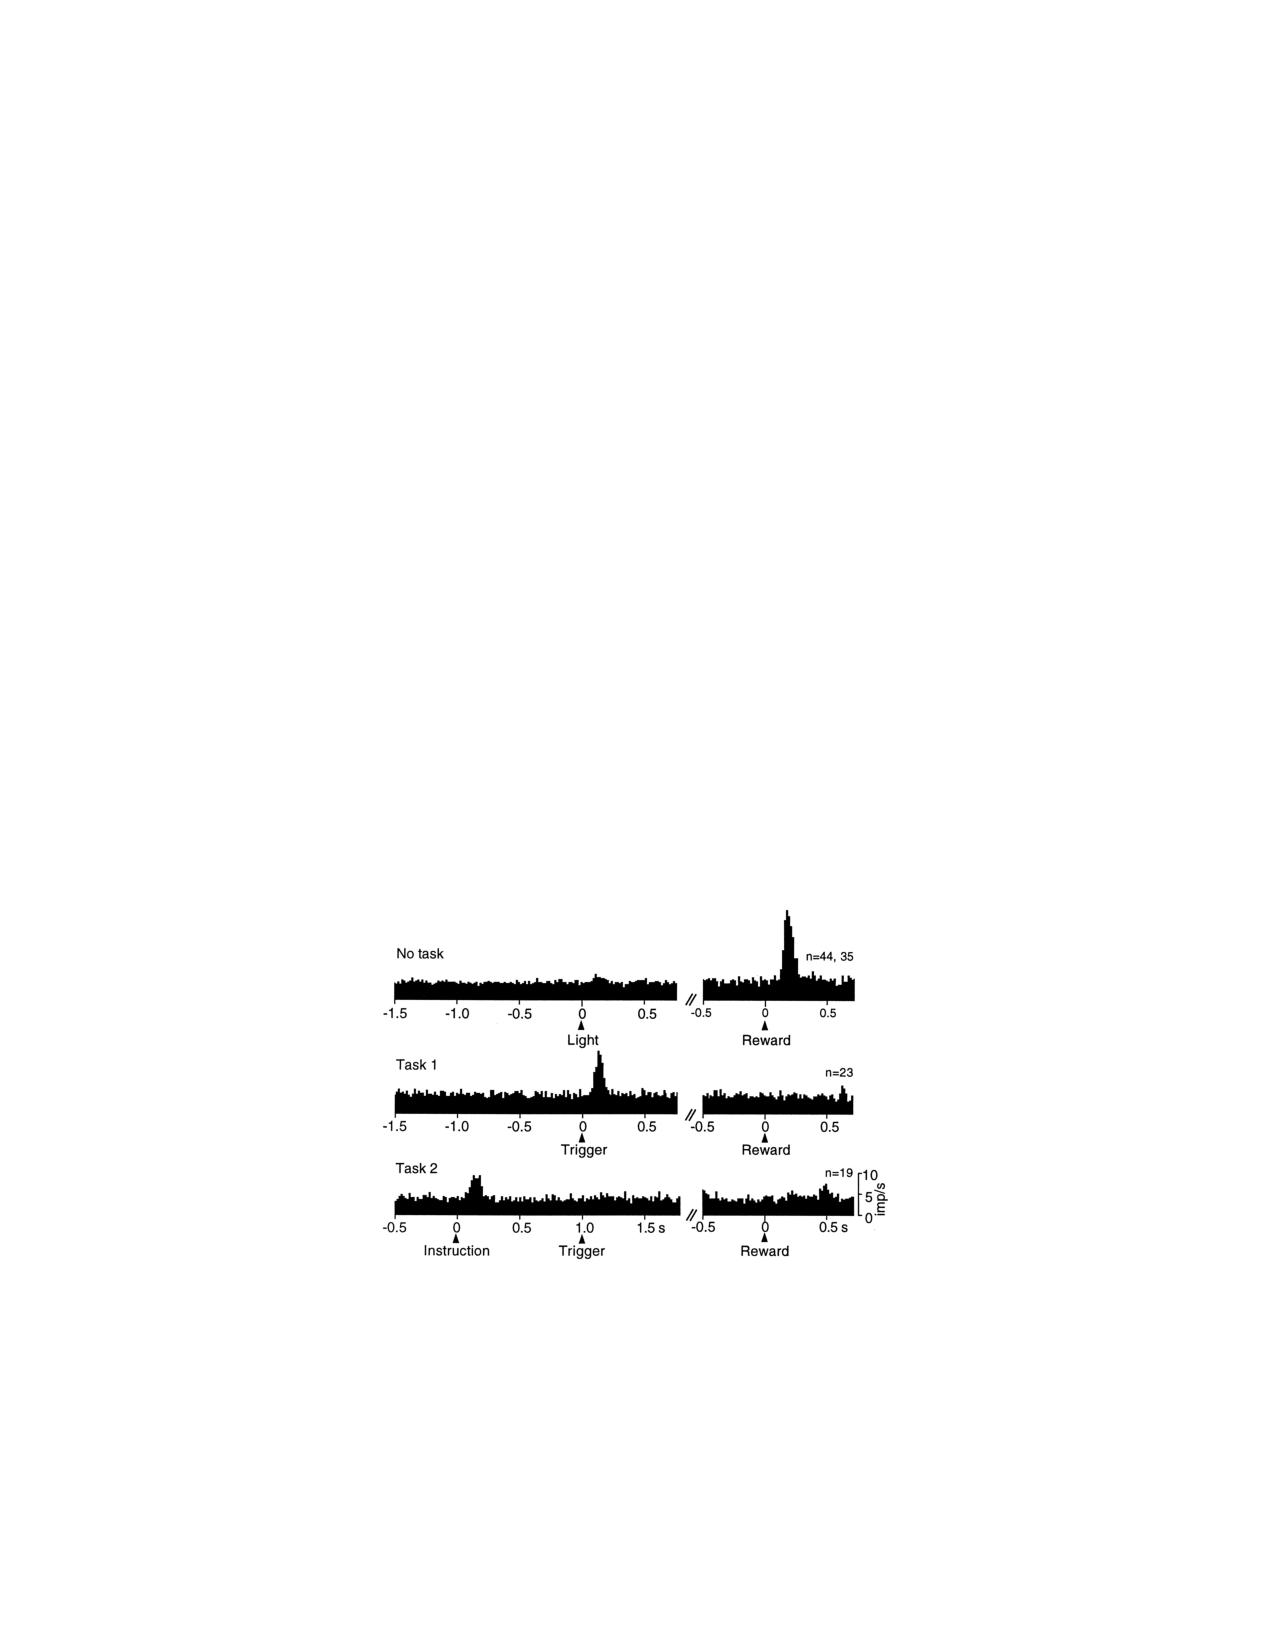
\includegraphics[width=0.5\linewidth]{chap12/fig_12_3}
	\caption{多巴胺神经元的反应从最初对初级奖励的反应转变为早期的预测刺激。
		这些是受监测的多巴胺神经元在小时间间隔内产生的动作电位数量的图,是所有受监测的多巴胺神经元(这些数据的范围从 23 到 44 个神经元)的平均值。
		上图:多巴胺神经元被意外输送的一滴苹果汁激活。
		中:通过学习,多巴胺神经元对奖励预测触发线索产生反应,并失去对奖励传递的反应。
		下图:通过在触发提示之前添加 1 秒的指令提示,多巴胺神经元将其反应从触发提示转移到更早的指令提示。
		来自舒尔茨等人。 (1995),麻省理工学院出版社。
		\label{fig:12_3}}
\end{figure}



在这项研究之后,同样的猴子接受了一项新任务的训练(Schultz、Apicella 和 Ljungberg,1993)。
在这里,猴子面对着两个杠杆,每个杠杆上方都有一盏灯。
点亮其中一个灯是一个“指令提示”,指示两个杠杆中的哪一个会产生一滴苹果汁。
在此任务中,指令提示在前一个任务的触发提示之前有 1 秒的固定间隔。
猴子学会了在看到触发提示之前不伸手,多巴胺神经元活动增加,但现在受监测的多巴胺神经元的反应几乎完全发生在较早的指令提示上,而不是触发提示上(图~\ref{fig:12_3},底部面板)。
当任务被很好地学习时,对指令线索做出反应的多巴胺神经元的数量再次大大减少。
在学习这些任务的过程中,多巴胺神经元活动从最初对奖励的反应转变为对早期预测刺激的反应,首先发展到触发刺激,然后发展到更早的指令提示。
随着反应时间提前,它会从后来的刺激中消失。
这种对较早奖励预测变量的反应的转变,同时失去对较晚预测变量的反应是 TD 学习的一个标志(例如,参见图~\ref{fig:12_4})。


\begin{figure}[!htb]
	\centering
	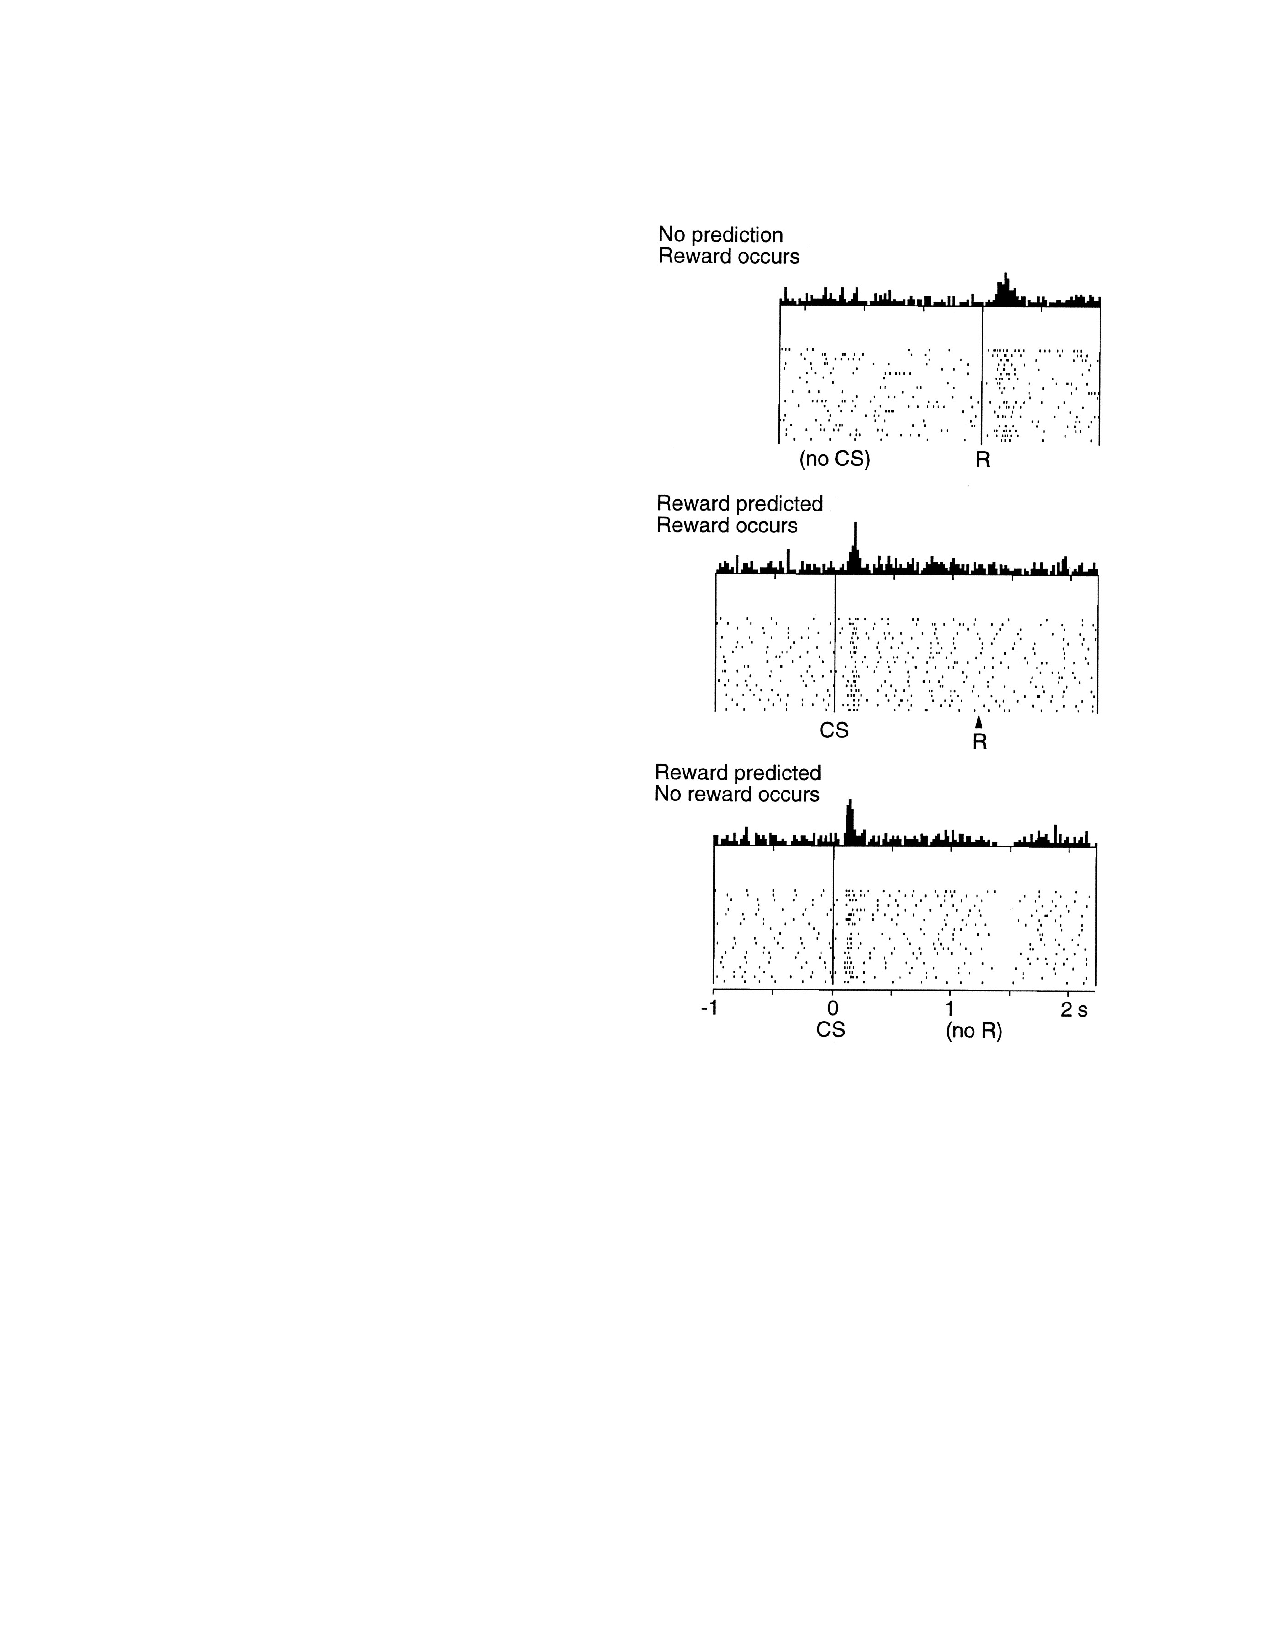
\includegraphics[width=0.5\linewidth]{chap12/fig_12_4}
	\caption{在预期奖励未能发生后不久,多巴胺神经元的反应就会降至基线以下。
		上图:一滴苹果汁的意外输送会激活多巴胺神经元。
		中:多巴胺神经元对预测奖励的条件刺激(CS)做出反应,但不对奖励本身做出反应。
		下图:当 CS 预测的奖励未能发生时,多巴胺神经元的活动在预期奖励发生后不久就会降至基线以下。
		每个面板的顶部显示了受监测的多巴胺神经元在指定时间附近的小时间间隔内产生的动作电位的平均数量。
		下面的光栅图显示了受监测的单个多巴胺神经元的活动模式;
		每个点代表一个动作电位。
		来自 Schultz、Dayan 和 Montague,《预测和奖励的神经基质》,科学,卷。 275,第 5306 期,第 1593-1598 页,1997 年 3 月 14 日。经美国科学促进会 (AAAS) 许可重印。
		\label{fig:12_4}}
\end{figure}


刚刚描述的任务揭示了多巴胺神经元活动与 TD 学习共有的另一个特性。
猴子有时会按错键,即按指示以外的键,因此得不到任何奖励。
在这些试验中,许多多巴胺神经元在奖励的通常传递时间后不久表现出其环率急剧下降至基线以下,并且这种情况发生时没有任何外部线索来标记通常的奖励传递时间(图~\ref{fig:12_4}) 。
不知何故,猴子在内部记录了奖励的时间。
(响应时间是需要修改最简单版本的 TD 学习的一个领域,以考虑多巴胺神经元响应时间的一些细节。我们将在下一节中考虑这个问题。)


上述研究的观察结果使舒尔茨和他的团队得出结论,多巴胺神经元对不可预测的奖励、最早的奖励预测因素做出反应,并且如果没有发生奖励或奖励预测因素,多巴胺神经元活性就会降低到基线以下 在预期的时间。
熟悉强化学习的研究人员很快认识到,这些结果与 TD 算法中 TD 误差作为强化信号的表现惊人地相似。
下一节将通过一个具体示例详细探讨这种相似性。


\section{时间差分误差/对应的多巴胺} \label{sec:td_dopamine}

本节解释 TD 误差与刚才描述的实验中观察到的多巴胺神经元的相位反应之间的对应关系。
我们研究了在类似上述任务的学习过程中如何变化,其中猴子首先看到指令提示,然后在固定的时间内必须正确响应触发提示才能获得奖励。
我们使用此任务的简单理想化版本,但我们比平常更详细,因为我们想强调 TD 误差和多巴胺神经元活动之间并行的理论基础。


第一个简化假设是代理已经学会了获得奖励所需的操作。
那么它的任务就是学习对其经历的状态序列的未来奖励的准确预测。
这是一个预测任务,或者更技术地说,是一个策略评估任务:学习固定策略的价值函数(第 4.1 和 6.1 节)。
要学习的价值函数为每个状态分配一个值,该值预测如果代理根据给定策略选择操作,该状态将遵循的回报,其中回报是所有未来奖励的(可能是折扣的)总和。
作为猴子情况的模型,这是不现实的,因为猴子可能会在学习正确行动的同时学习这些预测(就像学习策略和价值函数的强化学习算法一样,例如演员批评家算法),但这种场景比同时学习策略和价值函数的场景更容易描述。


现在想象一下,代理的经验分为多个试验,在每个试验中重复相同的状态序列,并且在试验期间的每个时间步上发生不同的状态。
进一步想象一下,预测的回报仅限于试验的回报,这使得试验类似于我们定义的强化学习事件。
当然,实际上,预测的回报并不局限于单次试验,试验之间的时间间隔是决定动物学到什么的重要因素。
对于时间差分学习来说也是如此,但这里我们假设回报不会通过多次试验累积。
鉴于此,舒尔茨及其同事进行的实验相当于强化学习的一个阶段。
(尽管在本次讨论中,我们将使用术语“试验”而不是“情节”,以便更好地与实验联系起来。)


像往常一样,我们还需要对状态如何表示为学习算法的输入做出假设,该假设会影响 TD 误差与多巴胺神经元活动的对应程度。
我们稍后讨论这个问题,但现在我们假设 Montague 等人使用相同的 CSC 表示。
(1996)其中,试验中每个时间步骤访问的每个状态都有一个单独的内部刺激。
这将流程简化为本书第一部分中介绍的表格案例。
最后,我们假设代理使用 TD(0) 来学习值函数 V ,该函数存储在所有状态下初始化为零的查找表中。
我们还假设这是一项确定性任务,并且折扣因子 非常接近 1,因此我们可以忽略它。


图~\ref{fig:12_5}~显示了 R、V 和 在该政策评估任务的几个学习阶段的时间过程。 
时间轴表示在试验中访问一系列状态的时间间隔(为了清楚起见,我们省略了显示各个状态)。
在每次试验中,奖励信号为零,除非智能体达到奖励状态(显示在时间线右端附近),此时奖励信号变为某个正数(例如 R?)。
TD 学习的目标是预测试验中访问的每个状态的回报,在这种未贴现的情况下,并且考虑到我们假设预测仅限于单个试验,那么 R 就是 R? 对于每个州。


\begin{figure}[!htb]
	\centering
	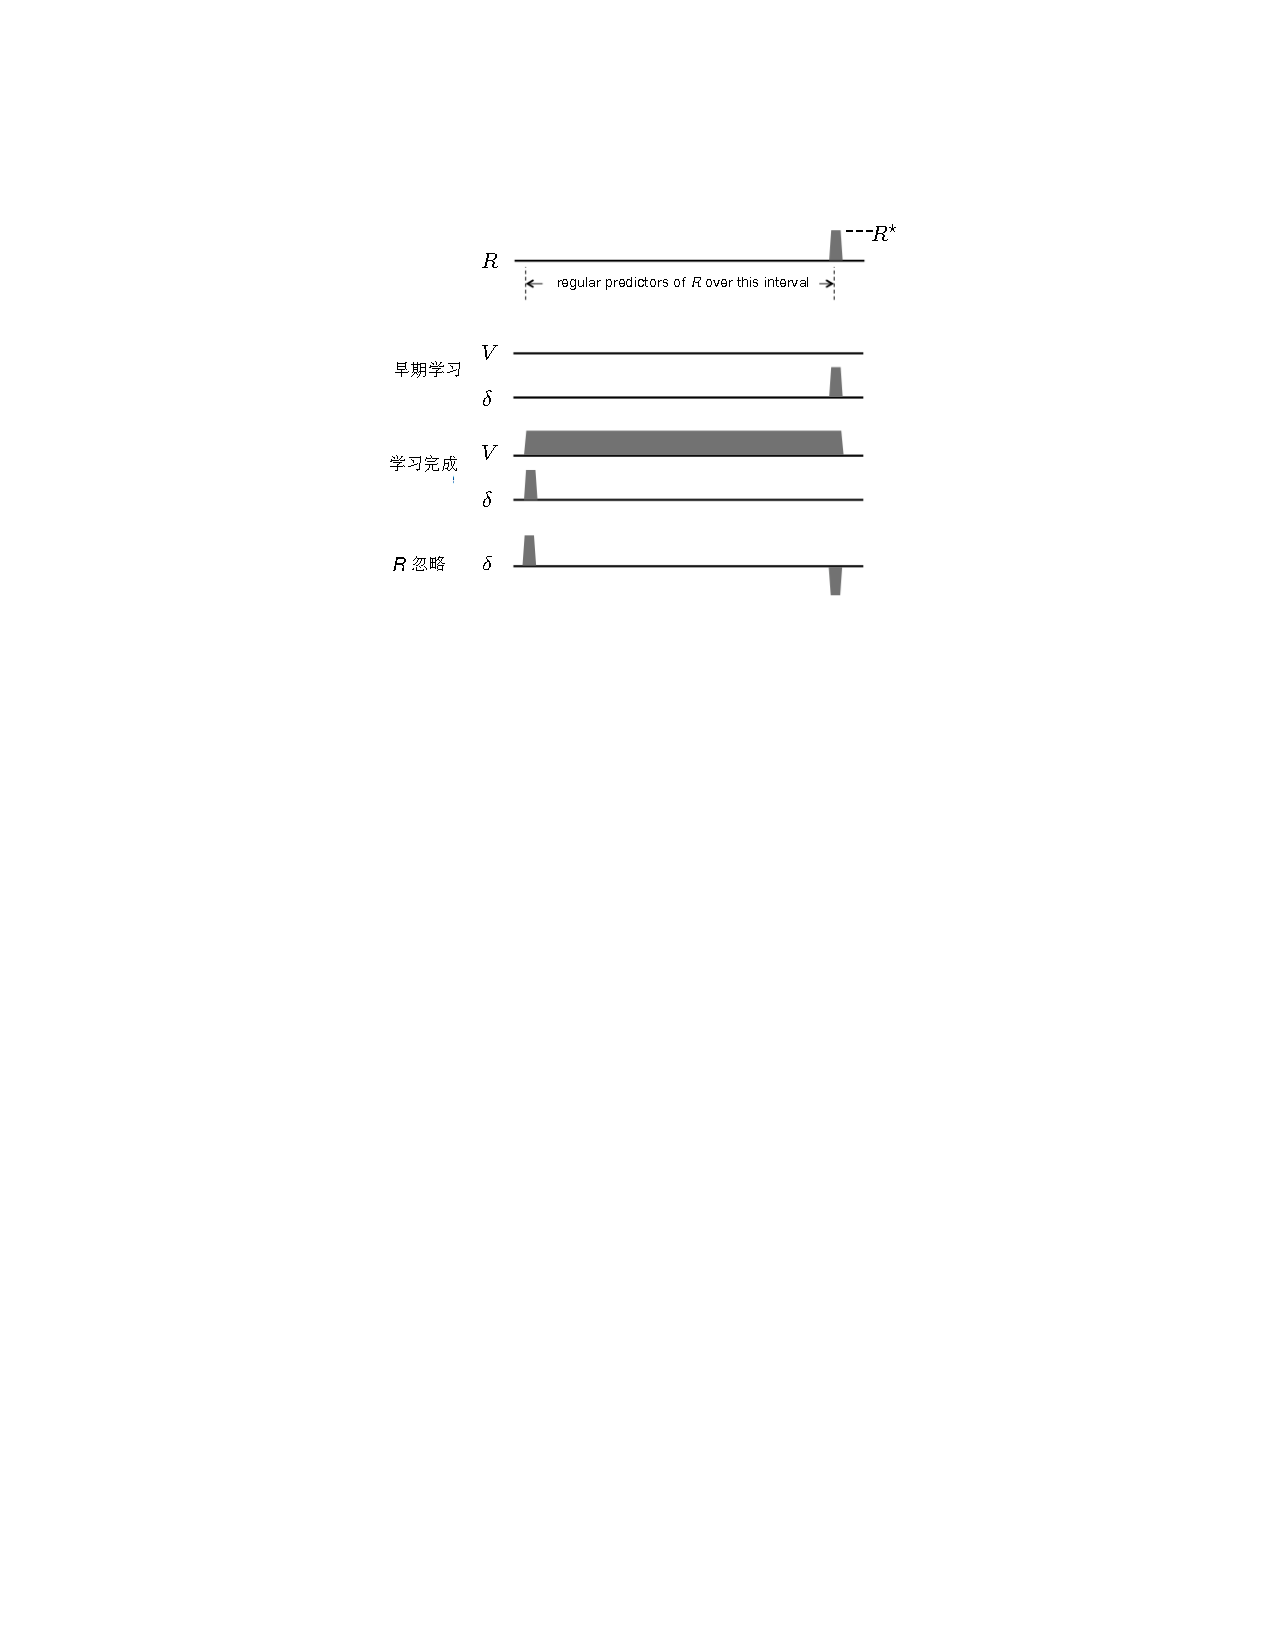
\includegraphics[width=0.5\linewidth]{chap12/fig_12_5}
	\caption{TD学习过程中TD误差的行为与多巴胺神经元的阶段性激活特征一致。
		(这里是时间 t 时的 TD 误差,即 t 1)。
		顶部:状态序列,显示为常规预测变量的区间,后面跟着非零奖励 R?。
		早期学习:初始值函数 V 和初始值,最初等于 R?。
		学习完成:价值函数准确地预测了未来的奖励,在最早的预测状态下为正,在非零奖励时=0。
		罗? 省略:当预测奖励被省略时,变为负数。
		请参阅文本以获取发生这种情况的完整解释。
		\label{fig:12_5}}
\end{figure}


奖励状态之前是一系列奖励预测状态,最早的奖励预测状态显示在时间线左端附近。
这就像试验开始时的状态,例如舒尔茨等人的猴子实验试验中由指令提示标记的状态。
(1993)如上所述。 它是试验中第一个可靠预测试验奖励的状态。
(当然,实际上,先前试验中访问的状态甚至是更早的奖励预测状态,但是因为我们将预测限制在单个试验中,所以这些状态不符合本次试验奖励的预测因子。
下面我们给出一个更令人满意的,但更多的 摘要,最早的奖励预测状态的描述。)试验中最新的奖励预测状态是紧接在试验的奖励状态之前的状态。
这是图~\ref{fig:12_5}~中时间线最右端附近的状态。
请注意,试验的奖励状态并不能预测该试验的回报:该状态的值将预测所有以下试验的回报,在这里我们假设在这个情景公式中为零。


图~\ref{fig:12_5}~显示了 V 的首次尝试时间课程,并标记为“早期学习”。 
因为除达到奖励状态外,整个试验过程中奖励信号为零,并且所有 V 值均为零,因此 TD 误差也为零,直到变为 R? 处于奖励状态。
这是因为 t 1 = Rt + Vt Vt 1 = Rt + 0 0 = Rt,在等于 R 之前它为零? 
当奖励发生时。 这里Vt和Vt·1分别是试验中在时间t和t·1访问的状态的估计值。
此学习阶段的 TD 误差类似于多巴胺神经元在训练开始时对不可预测的奖励(例如一滴苹果汁)的反应。



在第一个试验和所有后续试验中,TD(0) 更新发生在每个状态转换处,如第 6 章所述。这会连续增加奖励预测状态的值,并且增加从奖励状态向后传播,直到值 收敛到正确的回报预测。
在这种情况下(因为我们假设没有折扣)正确的预测等于 R? 对于所有奖励预测状态。
这可以在图~\ref{fig:12_5}~中看到,作为标记为“学习完成”的 V 的图,其中从最早到最新的奖励预测状态的所有状态的值都等于 R?。
最早奖励预测状态之前的状态值仍然很低(图~\ref{fig:12_5}~显示为零),因为它们不是可靠的奖励预测器。


当学习完成时,即当 V 达到其正确值时,与任何奖励预测状态的转换相关的 TD 误差为零,因为预测现在是准确的。
这是因为对于从奖励预测状态到另一个奖励预测状态的转变,我们有 t 1 = Rt + Vt 1 Vt 1 = 0 + R? = 0,对于从最新奖励预测状态到奖励状态的转变,我们有 t 1 = Rt+Vt 1 Vt 1 = R?+0 1R? = 0。
另一方面,从任何状态转换到最早的奖励预测状态的 TD 误差都是正的,因为该状态的低值与后续奖励预测状态的较大值之间不匹配。
事实上,如果最早奖励预测状态之前的状态值为零,那么在过渡到最早奖励预测状态之后,我们将得到 t 1 = Rt + Vt 1 Vt 1 = 0+R ? 0 = R?。 
图~\ref{fig:12_5}~中的“学习完成”图显示了最早奖励预测状态下的正值,而其他地方为零。


过渡到最早的奖励预测状态时的正 TD 误差类似于多巴胺对最早预测奖励的刺激的持续反应。
出于同样的原因,当学习完成时,从最新的奖励预测状态到奖励状态的转换会产生零 TD 误差,因为最新的奖励预测状态的值是正确的,会取消奖励。
这与观察结果相似,即与未预测的奖励相比,对完全预测的奖励产生阶段性反应的多巴胺神经元更少。


学习后,如果突然忽略奖励,则在通常的奖励时间,TD误差会变为负值,因为最新的奖励预测状态的值太高:t 1 = Rt + Vt 1 Vt 1 = 0 + 0 ??R? = }R?,如图~\ref{fig:12_5}~中“R 省略”图右端所示。
这就像在舒尔茨等人的实验中看到的那样,当预期奖励被忽略时,多巴胺神经元活动降低到基线以下。 (1993) 如上所述并如图~\ref{fig:12_4}~所示。


最早奖励预测状态的想法值得更多关注。
在上述场景中,由于经验被分为试验,并且我们假设预测仅限于单个试验,因此最早的奖励预测状态始终是试验的第一个状态。
显然这是人为的。
考虑最早的奖励预测状态的更一般方法是,它是不可预测的奖励预测器,并且可以有很多这样的状态。
在动物的一生中,许多不同的状态可能先于最早的奖励预测状态。
然而,由于这些状态后面经常跟随其他不预测奖励的状态,因此它们的奖励预测能力(即它们的值)仍然很低。
TD 算法如果在动物的整个生命周期中运行,也会更新这些状态的值,但更新不会持续累积,因为根据假设,这些状态中没有一个可靠地先于最早的奖励预测状态。
如果他们中的任何一个这样做了,他们也将获得奖励预测状态。
这也许可以解释为什么在过度训练的情况下,即使是试验中最早的奖励预测刺激,多巴胺反应也会减弱。
通过过度训练,人们会期望,即使是以前无法预测的预测状态也会被与早期状态相关的刺激所预测:动物在实验任务内外与其环境的相互作用将变得司空见惯。
然而,当引入一项新任务来打破这一惯例时,人们会看到 TD 错误再次出现,正如在多巴胺神经元活动中所观察到的那样。


上面描述的例子解释了为什么当动物在类似于我们例子的理想化任务的任务中学习时,TD误差与多巴胺神经元的阶段性活动共享关键特征。
但并非多巴胺神经元阶段性活动的每个属性都与 的属性如此完美地一致。
最令人不安的差异之一是当奖励早于预期出现时会发生什么。
我们已经看到,预期奖励的遗漏会在奖励的预期时间产生负预测误差,这对应于发生这种情况时多巴胺神经元的活动降低到基线以下。
如果奖励到达的时间晚于预期,那么它就是意外奖励并产生正预测误差。
TD 错误和多巴胺神经元反应都会发生这种情况。
但是,当奖励比预期更早到达时,多巴胺神经元不会做 TD 误差所做的事情|至少对于 Montague 等人使用的 CSC 表示来说是这样。 (1996)以及我们的例子。
多巴胺神经元确实会对早期奖励做出反应,这与正 TD 误差一致,因为预计奖励不会在那时发生。
然而,当奖励被预期但被忽略时,TD 误差为负,而与此预测相反,多巴胺神经元活动不会按照 TD 模型预测的方式降至基线以下(Hollerman 和 Schultz,1998)。
动物大脑中正在发生比简单地使用 CSC 表示进行 TD 学习更复杂的事情。



TD 误差和多巴胺神经元活动之间的一些不匹配可以通过为 TD 算法选择合适的参数值并使用 CSC 表示之外的刺激表示来解决。
例如,为了解决刚刚描述的早期奖励不匹配问题,Suri 和 Schultz(1999)提出了一种 CSC 表示,其中早期刺激引发的内部信号序列因奖励的出现而被取消。
Daw、Courville 和 Touretzky (2006) 提出的另一个建议是,大脑的 TD 系统使用在感觉皮层中进行的统计建模产生的表示,而不是基于原始感觉输入的简单表示。
Ludvig、Sutton 和 Kehoe (2008) 发现,使用微刺激 (MS) 表示的 TD 学习(图~\ref{fig:11_1})比使用 CSC 表示更好地控制早期奖励和其他情况下多巴胺神经元的活动。
Pan、Schmidt、Wickens 和 Hyland (2005) 发现,即使使用 CSC 表示,延长资格迹线也会改善多巴胺神经元活动某些方面的 TD 误差 t。
一般来说,TD 错误行为的许多细节取决于资格轨迹、贴现和刺激表示之间的微妙相互作用。
这些发现详细阐述并完善了奖励预测误差假说,但没有反驳其核心主张,即多巴胺神经元的阶段性活动被很好地表征为信号 TD 误差。


另一方面,TD 理论和实验数据之间还存在其他差异,这些差异不容易通过选择参数值和刺激表示来解决(我们在本章末尾的参考文献和历史评论部分提到了其中一些差异) ,并且随着神经科学家进行更加精细的实验,可能会发现更多的不匹配。
但奖励预测误差假说一直非常有效地发挥着催化剂的作用,有助于提高我们对大脑奖励系统如何运作的理解。
人们设计了复杂的实验来验证或反驳从该假设得出的预测,而实验结果反过来又导致了 TD 误差/多巴胺假设的完善和阐述。


这些发展的一个显着方面是,在完全不了解多巴胺神经元相关特性的情况下,从计算角度开发了与多巴胺系统特性密切相关的强化学习算法和理论| 请记住,TD 学习及其与最优控制和动态规划的联系早在任何揭示多巴胺神经元活动的 TD 性质的实验进行之前许多年就已经开发出来了。
这种计划外的对应关系尽管并不完美,但表明 TD 误差/多巴胺平行捕获了有关大脑奖励过程的重要信息。


除了解释多巴胺神经元阶段性活动的许多特征之外,奖励预测误差假说还将神经科学与强化学习的其他方面联系起来,特别是与使用 TD 误差作为强化信号的学习算法联系起来。
神经科学还远未完全理解多巴胺神经元的阶段性活动的回路、分子机制和功能,但支持奖励预测误差假说的证据,以及阶段性多巴胺反应是学习的强化信号的证据表明, 大脑可能会实现类似于 actor-critic 算法的算法,其中 TD 错误起着关键作用。
其他强化学习算法也是可能的候选者,但 actor-critic 算法特别适合哺乳动物大脑的解剖学和生理学,正如我们在下面两节中描述的那样。



\section{神经的参与者-评论家} \label{sec:neural_ac}


\section{参与者和评论家学习规则}


\section{享乐主义神经元}


\section{集体强化学习} \label{sec:collective_rl}


\section{大脑中基于模型的方法}


\section{成瘾}


\section{总结}










